% !TEX root = paper.tex
% !TEX encoding = UTF-8 Unicode

\begin{figure}
\begin{subfigure}[b]{\linewidth}
\begin{center}
\caption{Russian-English}
\label{fig:mean_adequacy_gain_ru}
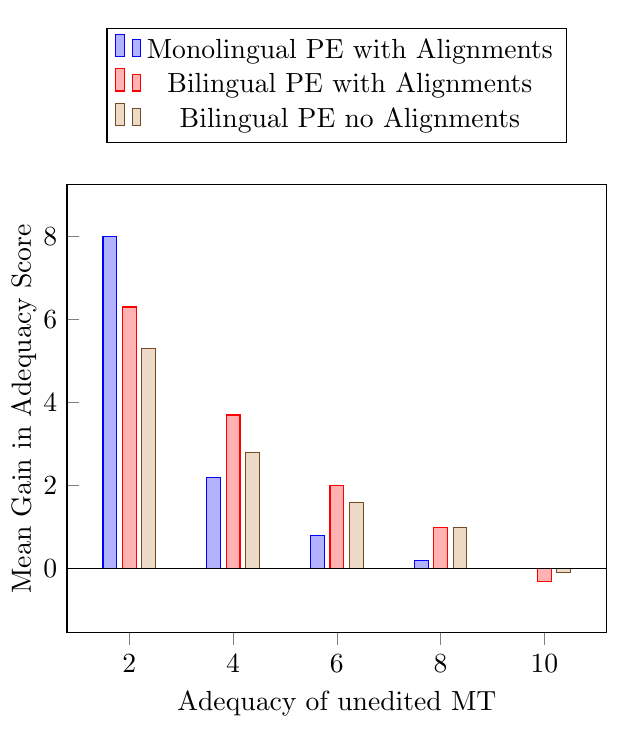
\begin{tikzpicture}[trim left={(-0.5,0)},trim axis right]
\begin{axis}[
	x tick label style={
		/pgf/number format/1000 sep=},
	ylabel shift={-0.15cm},
	ylabel=Mean Gain in Adequacy Score,
	xlabel={Adequacy of unedited MT},
%	ymin={0.1},
	enlargelimits=0.15,
	legend style={at={(0.5,1.35)},anchor=north},
	ybar,
	bar width=5pt,
	xtick pos=left,
	ytick pos=left,
%	ymin=0.0,
]
\addplot 
	coordinates {(2,8.0) (4,2.2)
		 (6,0.8) (8,0.2) (10,0)};

\addplot 
	coordinates {(2,6.3) (4,3.7)
		 (6,2.0) (8,1.0) (10,-0.3)};

\addplot 
	coordinates {(2,5.3) (4,2.8)
		 (6,1.6) (8,1.0) (10,-0.1)};

\addplot[black,sharp plot,update limits=false] 
	coordinates {(-1,0) (12,0)};

\legend{Monolingual PE with Alignments,Bilingual PE with Alignments,Bilingual PE no Alignments}
\end{axis}
\end{tikzpicture}
\end{center}
\end{subfigure}
\ \\ \ \\
\begin{subfigure}[b]{\linewidth}
\begin{center}
\caption{Spanish-English}
\label{fig:mean_adequacy_gain_es}
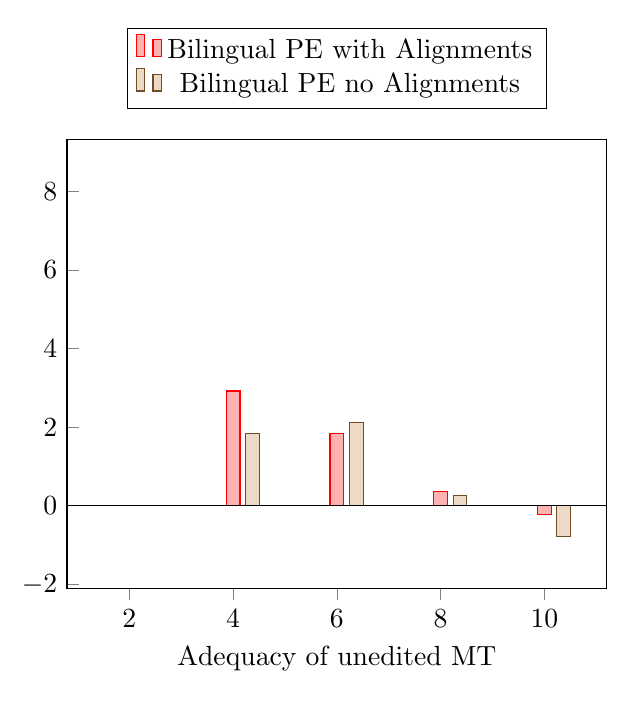
\begin{tikzpicture}[trim left={(-0.5,0)},trim axis right]
\begin{axis}[
	x tick label style={
		/pgf/number format/1000 sep=},
	ylabel shift={-0.15cm},
%	ylabel=Mean Gain in Adequacy Score,
	xlabel={Adequacy of unedited MT},
%	ymin={0.1},
	enlargelimits=0.15,
	legend style={at={(0.5,1.25)},anchor=north},
	ybar,
	bar width=5pt,
	xtick pos=left,
	xmin=2,
	ytick pos=left,
	ymax = 8,
%	ymin=0.0,
]
\addplot 
	coordinates {};

%	Gain with align	Gain w/o align
%2		
%4	2.92	1.84
%6	1.85	2.11
%8	0.36	0.25
%10	-0.22	-0.78

\addplot coordinates {(4,2.92) (6,1.85) (8,0.36) (10,-0.22) };
\addplot coordinates {(4,1.84) (6,2.11) (8,0.25) (10,-0.78) };

%\addplot coordinates {(4,2.6) (6,1.7272727272727273) (8,0.8181818181818182) (10,-0.07692307692307693) };
%\addplot coordinates {(4,2.0) (6,2.090909090909091) (8,0.9090909090909091) (10,-0.6153846153846154) };

\addplot[black,sharp plot,update limits=false] 
	coordinates {(-1,0) (12,0)};

\legend{Bilingual PE with Alignments,Bilingual PE no Alignments}
\end{axis}
\end{tikzpicture}
\end{center}
\end{subfigure}
\caption{Mean gain in adequacy score over unedited MT, categorized by the adequacy score of the unedited MT.}
\label{fig:mean_adequacy_gain}
\end{figure}
